
%%% Local Variables: 
%%% mode: latex
%%% TeX-master: t
%%% End: 

\chapter{研究背景}
\label{chap:background}

互联网应用如电子邮件、搜索、网络购物、社交网络、在线视频、网络地图等,
已经成为人们生活的一部分。
这些应用往往要为上亿用户服务,意味着互联网应用已变成如电力一样的社会公共服务,
而支撑拥有海量用户互联网应用的数据中心也成为如同发电厂一样的社会核心基础设施。

长尾延迟(Tail Latency)问题在数据中心中受到越来越多的关注,
造成长尾延迟的原因有很多,其中最为重要的原因就是资源共享带来的干扰。
由于没有行之有效的方案对干扰进行控制,目前典型的数据中心都使用隔离的方式来减小干扰,
这一方案虽然有效缓解了长尾延迟,但它也带来了资源利用率过低的问题,
现有商用数据中心的资源利用率普遍只有10\%-30\%左右,造成极大的浪费。
如何解决服务质量与资源利用率的问题是当前业界面临的重大挑战。

本章内容安排如下:首先介绍新计算模式对数据中心的挑战,
然后讨论现有数据中心技术的局限性,即服务质量与资源利率冲突的原因,
之后介绍针对该问题的相关工作,主要是软件架构、资源调度和体系结构支持三个方面的工作。

%服务质量(QoS)与资源利用率是数据中心运营时需要考虑的两个重要指标,前者严重影响用户
%体验,而后者直接与数据中心的运营成本相关。然而现有的计算机体系结构并没有为服务质量
%保障提供足够的支持,造成这两个指标在现实状况下存在冲突。为了保障用户体验,在实际系
%统部署时,会更多的考虑服务质量这一指标,造成数据中心的资源利用率严重低下,普遍只有
%10\%-30\%左右。基于这一现状,本文主要讨论如何设计一种高效的数据中心体系结构,使得
%数据中心在保障应用服务质量基础上,达到较高的资源利用率。
%

\section{新计算模式对数据中心的挑战}

\subsection*{计算模式1:以云计算为基础的移动计算}

随着移动设备(平板电脑、智能手机)计算能力不断增强、
成本不断降低以及无线通信技术的快速发展,移动计算时代已经来临。
如表\ref{tab:ganter-sales}所示,
Gartner调研数据显示平板电脑和手机(包含智能手机和普通手机)销量不断增加,
与此同时PC销量则不断下降。
而IDC预测到2015年智能手机销量将超过14亿部,
占所有个人计算设备(包括PC、平板电脑和智能手机等)69\%的销量份额。

% Gartner关于电脑与移动设备销量的统计 
\begin{table}[htb]
  \centering
  \begin{minipage}[t]{0.9\linewidth}
  \caption[全球个人计算设备市场销量统计]{全球个人计算设备市场销量统计(单位:千部)}
  \label{tab:ganter-sales}
    \begin{tabular*}{\linewidth}{lrrrrr}
      \toprule[1.5pt]
      {\heiti 设备类型} & {\heiti 2012年} & {\heiti 2013年} & {\heiti 2014年} & {\heiti 2015年} & {\heiti 2016年} \\
      \midrule[1pt]
      PC(台式机、笔记本) &   341,273 &   296,131 &   279,000 &   259,000 &   248,000 \\ 
      超级本               &     9,787 &    21,517 &    39,000 &    62,000 &    85,000 \\ 
      平板电脑             &   120,203 &   206,807 &   216,000 &   233,000 &   259,000 \\ 
      手机                 & 1,746,177 & 1,806,964 & 1,838,000 & 1,906,000 & 1,969,000 \\ 
      其他移动设备         &       --- &     2,981 &     6,000 &     9,000 &    11,000 \\
      %总计                 & 2,217,440 & 2,334,400 & 2,378,000 & 2,470,000 & 2,572,000 \\
      \bottomrule[1.5pt]
    \end{tabular*}\\[2pt]
    \footnotesize
    数据来源:Gartner,2012年(http://www.gartner.com/newsroom/id/2610015),
    2013年(http://www.gartner.com-\\/newsroom/id/2791017),
    2014-2016年(http://www.gartner.com/newsroom/id/2954317)
  \end{minipage}
\end{table}

移动计算的快速发展带来新的计算模式:
移动设备通过无线通信与运行在云计算平台的各类应用服务进行交互。
据可靠消息,目前一些主要的互联网公司(如Facebook和Baidu等)均表示,
来自移动设备的请求已占到40\%以上,并且仍在快速增长,很快将超过PC。
随着4G时代的到来,这种移动计算模式将成为未来的主流。

快速增长的移动计算需求对云计算平台的核心------数据中心带来了严峻的挑战。
这种交互式计算模式,快速的服务响应时间是衡量服务质量(Quality-of-Service,QoS)的关键指标,
是让用户满意、留住用户的关键。有研究表明,如果服务响应时间增加,公司收入就会减少。
例如,2009年微软在Bing搜索引擎上也开展实验,发现当服务响应时间增加到2000ms时,
每个用户带给企业的收益更是下降了4.3\%。
由于该实验对公司产生了负面影响,最终不得不被终止\cite{bing:2009}。
Amazon也发现其主页加载时间每增加100ms就会导致销售额下降1\% 。
而Google更是发现当搜索结果返回时间从0.4s增加到0.9s时,广告收入下降了20\%。

\begin{figure}
\begin{minipage}{0.48\textwidth}
  \centering
  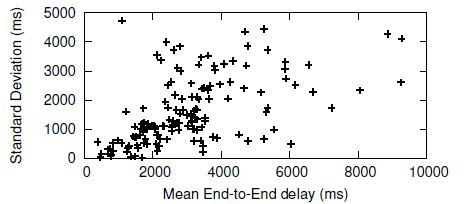
\includegraphics[height=5cm]{bg/end2end-delay}
  \caption[北美移动应用用户感知时延分布]{北美移动应用用户感知时延分布:平均延迟超过2秒且具有很大的波动性}
  \label{fig:end2end-delay}
\end{minipage}\hfill
\begin{minipage}{0.48\textwidth}
  \centering
  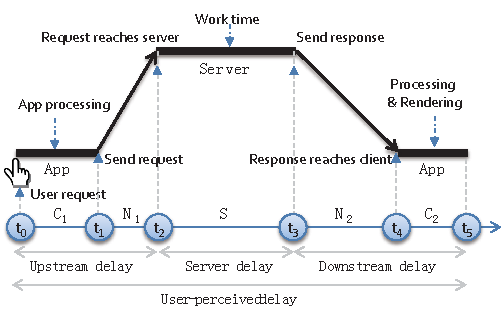
\includegraphics[height=5cm]{bg/interact-apps}
  \caption[一个典型的交互式请求的5个阶段]{一个典型的交互式请求的5个阶段:
    C1$\rightarrow$N1$\rightarrow$S$\rightarrow$N2$\rightarrow$C2\cite{timecard:2013}}
  \label{fig:interact-apps}
\end{minipage}
\end{figure}

移动计算的响应时间仍然存在很大的提升空间。
如图\ref{fig:end2end-delay}所示,微软公司实验数据表明在北美网络环境下,
交互式移动设备的平均时延超过2秒,而且存在较大的波动性。
图\ref{fig:interact-apps}显示典型移动交互式应用的用户请求时延分为5个阶段,
最近研究\cite{timecard:2013}表明其中数据中心服务器的处理时延S约为1.2秒,占60\%。
随着4G网络的来临,数据中心将面临更大规模用户数据的处理请求。
因此,如何快速处理和及时响应移动计算请求将成为数据中心设计的核心目标之一。


\subsection*{计算模式2:面向大数据处理的实时计算}

大数据时代的到来使大数据处理架构受到越来越多的关注。
2013年底中国计算机学会(CCF)大数据专家委员会发布的
《2014年大数据发展趋势十大预测》报告中,
来自学术界、产业界、海外、跨界特邀和政府的122位专家们普遍认为,
Hadoop/MapReduce框架一统天下的模式将被打破,
而实时流计算、分布式内存计算、图计算框架等将并存。

\begin{figure}[H]
  \centering
  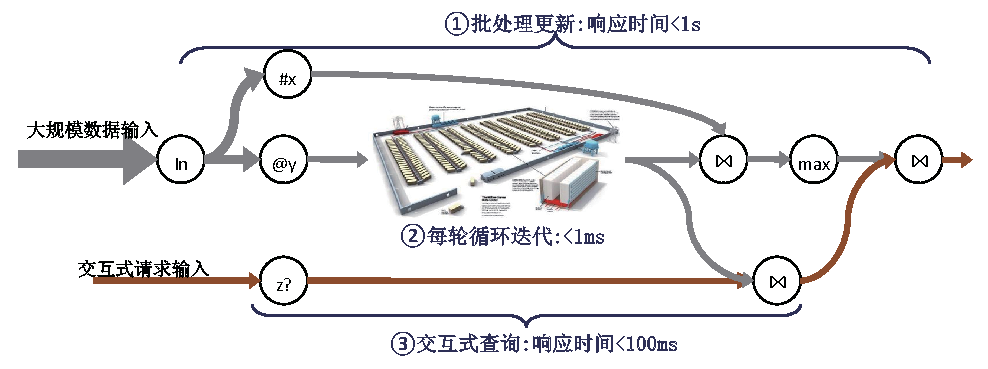
\includegraphics[height=6cm]{bg/batch-apps}
  \caption{典型的3类大数据处理需求以及相应的响应时间要求}
  \label{fig:batch-apps}
\end{figure}


大数据处理对数据中心和处理架构提出新的挑战,
图\ref{fig:batch-apps}显示了典型的大数据处理需求:
首先需要支持数据的批处理更新模式(<1s);
其次数据处理会分解为多次迭代计算(<1ms);
再次还要支持实时计算模式,处理多用户的交互式查询请求(<100ms);
而这些处理所需要的数据存放在同一个数据中心。
搜索引擎是一个典型的例子,既需要对大规模网页进行内容处理,迭代计算页面的pagerank,
还需要处理大量用户的关键字查询请求。

尽管大数据处理希望能将各种处理集成在一个处理架构上,然后部署在一个数据中心。
但如果实时计算与企业营收相关,比如搜索引擎、在线购物等在线服务应用,
那么正如微软Bing实验所示,这些面向在线服务应用的实时计算的服务质量就非常关键
(以下用``在线应用''代表``实时计算'')。
为了保障在线应用的服务质量,
主流互联网企业一般将在线应用与大规模批处理作业分别部署到不同的数据中心,
以减少批处理作业对在线应用的干扰。
但由于用户查询请求数量具有显著的随时间变化的波动性,
这种分离作业、单独部署的模式会导致在线应用数据中心的资源平均利用率很低。
如图\ref{fig:google-util-2013}所示,Google的两类数据中心CPU利用率相差达2.5倍,
在线应用数据中心资源利用率仍有很大提升空间。


%% 典型的数据中心一般有5~10万台服务器组成,建设与运行维护成本往往高达几十亿人民
%% 币。然而出于保障应用服务质量的原因,现有数据中心只能维持较低的资源利用率,导致大量
%% 资源浪费。因此,本项目总体研究目标为如何设计高效通用数据中心体系结构:``通用''表
%% 示数据中心可同时运行各种不同类型应用;``高效''表示数据中心能在保障延迟敏感应用的服
%% 务质量基础上,达到较高的资源利用率(CPU利用率>60\%)。
%% 
%% 典型的数据中心一般有5~10万台中低端服务器组成,这些服务器通过内部网络互连,一起协同
%% 运行互联网应用为海量用户服务。因为这类数据中心规模很大,往往部署在大型仓库级别的机
%% 房,从应用角度来看就如同一台计算机,因此也被称为
%% ``仓库级计算机(Warehouse-Scale Computer)'' \cite{WSC}。
%% 国内外著名的互联网公司往往拥有多个数据中心,服务器数量达到数十万甚
%% 至上百万台。例如,谷歌(Google)的数据中心服务器数量已经超过百万台为全球用户提供
%% 搜索、邮件、地图等服务[2];亚马逊(Amazon)仅EC2就部署了约50万台服务器提供云计算服
%% 务[3];据可靠消息,国内腾讯公司也拥有约30万服务器为用户提供各种互联网服务。
%% 
%% 尽管目前互联网企业的数据中心已经颇具规模,但一个趋势是未来数据中心还将持续发展。一
%% 方面互联网用户数量仍在不断增长,目前全球已有24亿网络用户,但很多机构预测未来全球还
%% 将新增30亿网民融入到互联网[4],这会对数据中心的数量和规模都提出更多需求。另一方面快
%% 速发展的移动终端已超越个人计算机(PC),成为终端计算设备的主流。由于移动设备性能相对
%% 较低、存储容量较小,将计算与存储转移到数据中心的需求也变得越来越强烈。因此数据中心作
%% 为基础设施也会日益重要。


\section{现有数据中心技术的局限性}

通过上述分析可知,移动计算与实时计算均对快速响应用户请求提出了强烈的需求。
而当前数据中心为了保障用户请求的服务质量,
不得不通过采用牺牲资源利用率、保留过量资源的方式。
以Google的数据中心为例,
图\ref{fig:google-util-2006}显示了2006年Google数据中心平均CPU利用率为30\%左右。
但到2013年,虽然Google将数据中心分为了两类,并且批处理数据中心已经能达到75\%的CPU利用率,
但在线应用数据中心仍停留在30\%。
Google的数据中心技术一直处于领先地位,
与之相比,国内一些主流互联网企业在线应用数据中心CPU利用率一般都低于20\%,
有的甚至低于10\%,仍然存在很大的提升空间。

% Google数据中心利用率 
\begin{figure}
\begin{minipage}{0.57\textwidth}
  \centering
  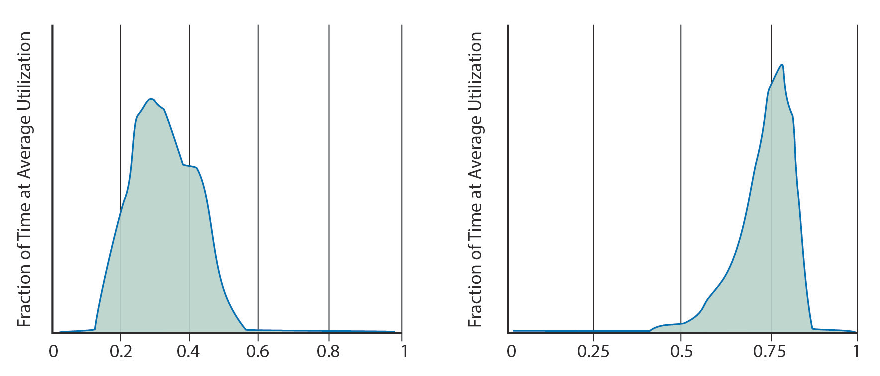
\includegraphics[height=4cm]{bg/google-util-2013}
  \caption[Google数据中心CPU利用率分布(2013年)]
    {Google数据显示2013年1至3月在线应用数据中心CPU利用率平均只有30\%(左图),
     而批处理作业数据中心则能达到75\%的利用率(两个数据中心均为2万台服务器)\cite{barroso_datacenter_2013}}
  \label{fig:google-util-2013}
\end{minipage}\hfill
\begin{minipage}{0.39\textwidth}
  \centering
  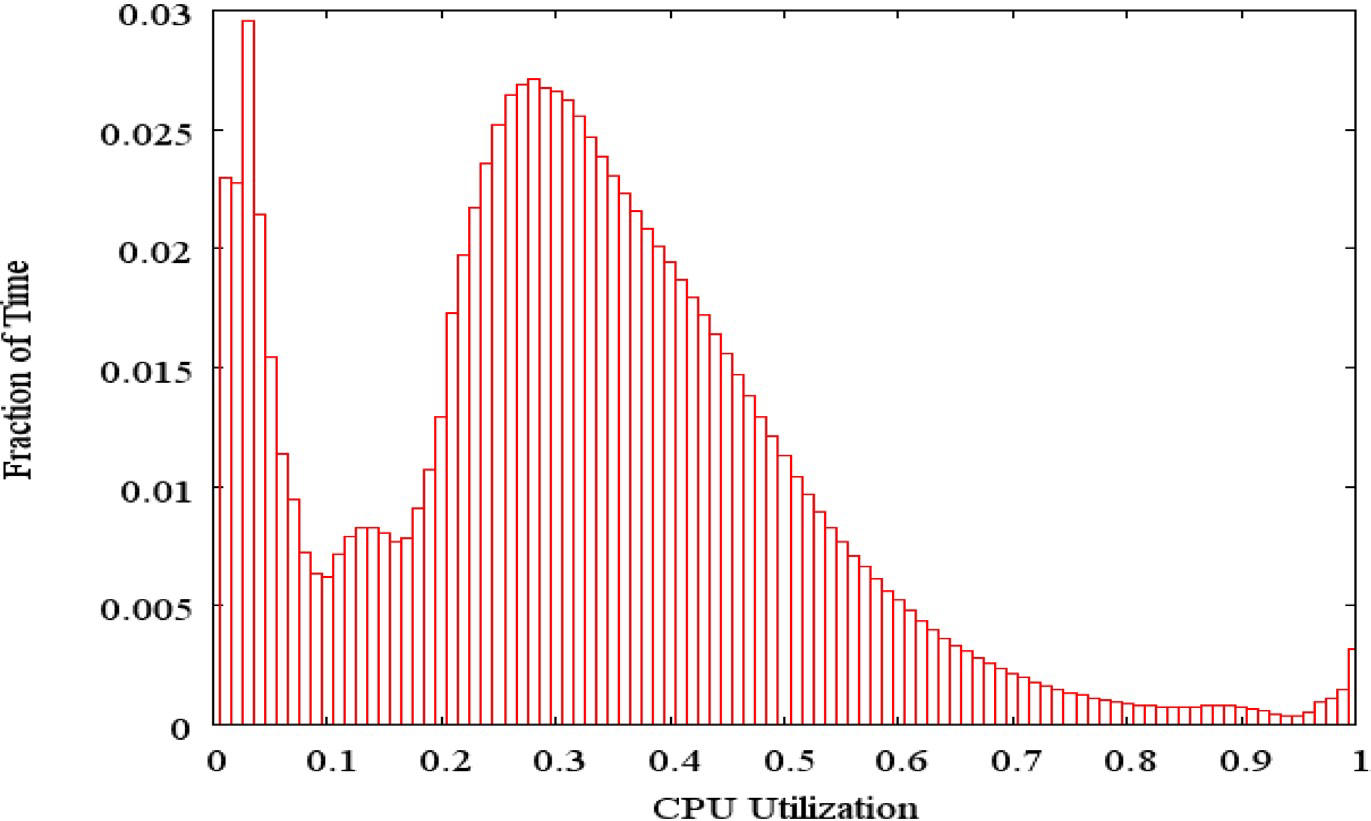
\includegraphics[height=3.5cm]{bg/google-util-2006}
  \caption[Google数据中心CPU利用率分布(2006年)]
    {Google在2006年数据中心(5000台服务器)6个月的CPU利用率分布\cite{barroso_datacenter_2009}}
  \label{fig:google-util-2006}
\end{minipage}
\end{figure}

尽管在线数据中心资源利用率只有30\%,但Google已经观察到严峻的长尾延迟现象:
最慢的1\%$\sim$10\%请求处理时间远大于所有请求的平均响应时间。
如图\ref{fig:google-resptime-dist}所示,Google某后台服务延迟响应时间平均仅为5$\sim$6ms,
但是却有相当一部分请求响应时间超过了100ms\cite{Krushevskaja:2013}。
而长尾延迟现象在数据中心环境下会被更进一步放大,
因为一个用户请求需要几百上千台服务器共同完成,只要有一台服务器的处理速度受到干扰,
就会导致整个请求的处理时间增加。
Google的Jeff Dean在2012年Berkeley的报告\cite{dean_achieving_2012}中
就指出了长尾现象的严重性:假设一台机器处理请求的平均响应时间为1ms,
有1\%的请求为长尾处理时间会大于1秒(99th-Percentile);
如果一个请求需要由100个这样的节点一起处理,那么就会出现63\%的请求响应时间大于1秒
(如图\ref{fig:long-tail-amplify}所示)。

造成在线应用数据中心资源利用率低和长尾延迟现象的核心原因是,
现有数据中心技术无法在多应用混合运行时消除应用间干扰,以实现不同应用之间的性能隔离。
Google的Jeff Dean与Luiz Barroso在2013年2月的《Communication of the ACM》上撰文
``The Tail at Scale''\cite{dean_tail_2013}分析确认导致长尾延迟的首要原因就是资源共享,
包括体系结构层次的CPU核、Cache、访存带宽、网络带宽等,而干扰不仅来自应用,
还会来自系统软件层次的后台守护作业、监控作业、共享文件系统等。
Google在分布式架构和软件层次采用了多种缓解长尾延迟的技术,
包括操作系统容器隔离技术\cite{cgroup}、应用优先级管理\cite{google_trace}、
备份请求\cite{dean_achieving_2012}、同步后台管理进程\cite{dean_achieving_2012}等,
取得了一定的效果,但却无法消除硬件体系结构层次上的应用之间的干扰,
导致仍然会出现图\ref{fig:google-resptime-dist}这样的长尾延迟。

\begin{figure}
\begin{minipage}{0.44\textwidth}
  \centering
  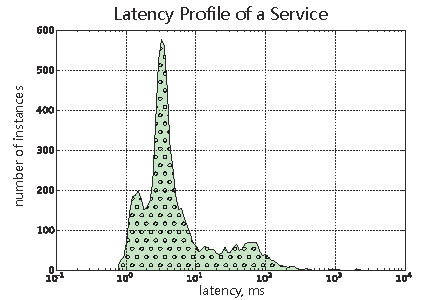
\includegraphics[width=\textwidth]{bg/google-resptime-dist}
  \caption[Google某后台服务的响应时间分布]{Google某后台服务的响应时间分布\cite{Krushevskaja:2013}}
  \label{fig:google-resptime-dist}
\end{minipage}\hfill
\begin{minipage}{0.52\textwidth}
  \centering
  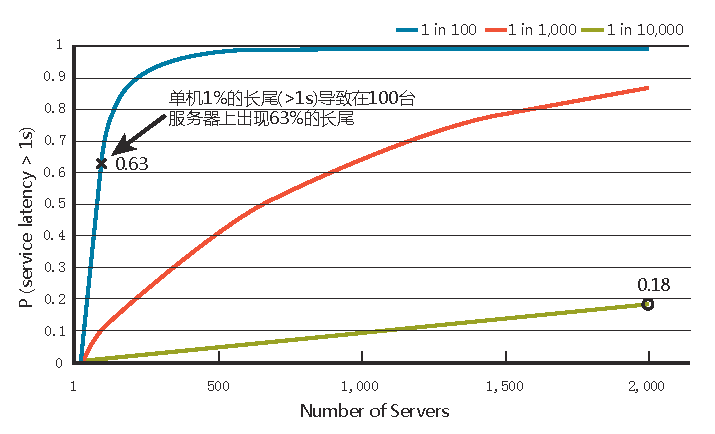
\includegraphics[width=\textwidth]{bg/long-tail-amplify}
  \caption[长尾延迟放大效应]{长尾延迟放大效应\cite{dean_tail_2013}}
  \label{fig:long-tail-amplify}
\end{minipage}
\end{figure}

因此,现有数据中心处于``无管理的资源共享''状态,这
导致出现资源利用率与应用服务质量之间的矛盾:
一方面通过多个应用同时在数据中心部署实现资源共享能有效提高资源利用率,
但另一方面多个应用共享资源又会出现相互干扰严重影响应用的服务质量。
因此,目前企业不得不采用预留额外资源以保障延迟敏感的在线应用服务质量,
这导致很低的数据中心利用率。
而且随着多核技术的发展,单个服务器内的资源越来越多,
其上混合部署的应用数目也在不断增加,更会加剧这种矛盾。

\section{相关工作}

随着应用数量与规模的不断增加,数据中心所需要的服务器数量也在飞速增长中。
而受到电力供应、冷却系统以及占地面积等客观因素的影响,
服务器规模并不能够无限制的扩大,
服务器融合(Server Consolidation)成为当前应用部署的主流技术。
本节首先介绍当前常见的服务器融合技术,并对比其在资源、性能等方面的隔离性;
然后介绍在这种服务器融合的共享环境下,已有的服务质量与资源管理的相关工作;
最后对比网络领域中解决服务器质量与资源管理的方案,
讨论将其应用于计算机体系结构中的可行性。

\subsection{服务器融合技术}

通过考查现代数据中心的应用架构,可以发现其中大部分架构都符合``数据复用模型'',
即多个应用程序协同工作,每个应用只对数据进行部分处理,然后交给下级应用程序,
这些应用程序最终组合完成一个服务功能,提供给最终用户。
通过这种方式形成的复杂应用架构,由于在兼容性、性能或安全等多方面的原因,
各个模块通常不能很好的在一台服务器内工作,而是需要多台服务器进行部署,
大量这样的多服务器应用给数据中心的维护工作带来了很大的挑战。
从另一方面,应用与服务器规模的不断增长,
数据中心在占地、电力消耗、冷却系统等方面也产生了极大的压力,
但服务器资源利用率过低的问题,造成数据中心整体的效率十分低下。
为解决这一问题,许多软硬件厂商都提出了自己的方法与技术,
将应用部署到更少的物理服务器中,实现高效可管理的服务器融合,
其中虚拟化、硬件分区与基于容器的轻量级虚拟化是三种目前应用最为广泛的服务器融合技术。

% 硬件分区
虚拟化技术最初由IBM在20世纪60年代提出,当时提出虚拟化的目的是为了提供系统的向后兼容性,
以简化用户编程,而后虚拟化一直是大型机基本的使用方式。
在此基础上IBM提出了逻辑分区(LPAR)\cite{IBM_LPAR:2007}技术,
该技术使得一台计算机能够像两台或更多有独立计算机一样运行,
为服务器融合提供了平台支持,
其他一些厂商如Hitachi\cite{hitachi-lpar}和Sun(Oracle)\cite{LDom}也提供了类似的解决方案。

% 软件虚拟化
VMware首先将虚拟化技术引入到基于x86的PC服务器领域,
由于当时x86架构并没有提供任何虚拟化的支持,
VMware使用二进制翻译\cite{vmware-compare-hw-sw:2006}
的方式实现操作系统内核中不支持虚拟化的指令执行,
如图\ref{fig:compare-of-virt}(a)所示,实现对用户操作系统透明的虚拟化方案。
这种基于二进制翻译的全虚拟化方案性能存在问题,
因此Xen提出了半虚拟化(para-virtualization)\cite{barham_xen_2003}的概念,
通过修改客户机操作系统,直接使用Hypercall的方式调用hypervisor
(如图\ref{fig:compare-of-virt}(b)所示),提高系统性能。
在虚拟化产业发展起来后,各个硬件厂商分别推出新的硬件功能以更好的支持虚拟化,
如Intel的VT-x技术和AMD的AMD-V技术,如图\ref{fig:compare-of-virt}(c)所示,
硬件辅助虚拟化逐渐成为主流。
随着虚拟化技术性能的不断提高,当前在PC服务器领域,
虚拟化技术已经成为数据中心内被普遍使用的技术。

\begin{figure}[t]
  \centering
  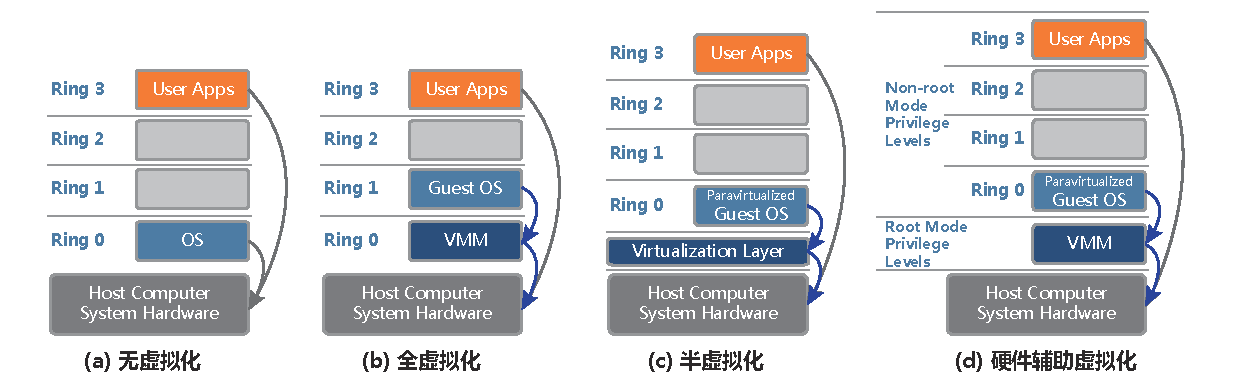
\includegraphics[width=\textwidth]{bg/compare-of-virtualization}
  \caption[三种不同类型虚拟化技术的对比]{三种不同类型虚拟化技术的对比:
    (a)无虚拟化,直接执行用户与OS请求;
    (b)全虚拟化,直接执行用户请求,二进制翻译执行OS请求;
    (c)半虚拟化,直接执行用户请求,修改GuestOS通过Hypercall实现特权指令;
    (d)硬件辅助虚拟化,直接执行用户请求,硬件支持OS特权指令直接陷入到VMM。}
  \label{fig:compare-of-virt}
\end{figure}

%轻量级虚拟化
基于容器的轻量级虚拟化是另一种流行的服务器融合技术,
与虚拟机抽象类似,不同容器之间以及容器与主机操作系统之间是相互隔离的,
但它们共享一份操作系统内核,可以有效的提高资源利用率。
以Docker为例(如图\ref{fig:docker-overview}),
用户的应用与依赖的运行时环境被打包为一个容器,
容器之间使用Linux内核的LXC\cite{lxc}机制实现名字空间隔离,
同时使用Control Group\cite{cgroup}实现资源控制。
与虚拟化技术相比,容器技术最大的优点是它具有更少的资源占用,以及更快的启动时间,
因此也被普遍运行在数据中心场景中。

\begin{figure}[htb]
  \centering
  \begin{minipage}{0.75\textwidth}
    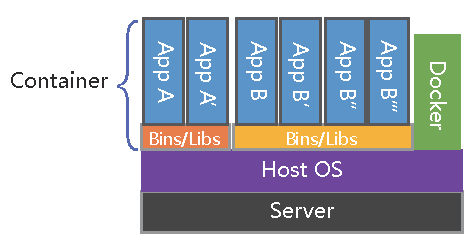
\includegraphics[width=0.75\textwidth]{bg/docker-overview}
    \caption[容器虚拟化结构示意(Docker)]{容器虚拟化结构示意(Docker):
      容器中包含应用及其依赖的运行时环境,容器之间相互隔离但它们共享同一份操作系统内核。}
    \label{fig:docker-overview}
  \end{minipage}
\end{figure}

% TODO:各种服务器融合技术对比


\subsection{资源管理与服务质量保障}

表\ref{tab:contention}列出了部分尝试消除各个层次竞争点的工作,
Google和Twitter等互联网公司也正在尝试改进数据中心管理系统架构,
实现服务器资源利用率与应用服务质量之间的平衡,
一些典型系统包括:Borg\cite{borg:2015}、Omega\cite{Schwarzkopf_omega_2013}和
Mesos\cite{Hindman:2011:Mesos}。
另外一些研究工作尝试使用分布式技术或操作系统内核优化技术实现应用服务质量保障,
如多级优先级策略\cite{google_trace}、
调度方法\cite{delimitrou_paragon:_2013, delimitrou_quasar:_2014,  mars_heterogeneity_2011,
kozyrakis_reconciling_2014, Novakovi:ATC2013}、
backup-request\cite{dean_tail_2013},cgroup\cite{cgroup}和容器技术\cite{lxc}。 
本节主要关注节点内资源管理与服务质量保障的相关研究,包括软件和硬件两个方面。

\begin{table}[hb]
  \centering
  \caption{资源管理与服务质量保障相关工作中识别出的竞争点}
  \label{tab:contention}
  \begin{tabular}{p{0.2\textwidth}p{0.7\textwidth}}
    \toprule[1.5pt]
      {\heiti 层次}     & {\heiti 竞争点}                                                                                      \\
    \midrule[1pt]
      数据中心          & Global file system \cite{dean_tail_2013}                                                                        \\
      应用层            & Background daemon \cite{dean_tail_2013}, backup job \cite{yu_profiling_2011,dean_tail_2013}                     \\
      网络协议栈        & Nagle's algorithm, limited buffers, delayed ACK caused RTO \cite{yu_profiling_2011},
                          TCP congestion control \cite{alizadeh_data_2010,dong_less_2013},
                          packet scheduling \cite{vamanan_deadline-aware_2012,wilson_better_2011,zats_detail:_2012,hong_finishing_2012},
                          kernel sockets \cite{kozyrakis_reconciling_2014}                                                                \\
      操作系统内核      & Lock contention \cite{Kapoor:2012:Chronos}, context switch, kernel scheduling,
                          SMT load imbalance and IRQ imbalance \cite{kozyrakis_reconciling_2014}                                          \\
      虚拟化层          & Virtual machine scheduling \cite{Xu:2013:Bobtail:,wang_impact_2010, Xu:2013:SMALL},
                          network bandwidth \cite{wang_impact_2010,shieh_sharing_2011,Xu:2013:SMALL,jeyakumar_eyeq:_2013}                 \\
      硬件              & Shared caches \cite{kozyrakis_reconciling_2014,Tang:2011:ISCA,kasture_ubik:_2014,sanchez_vantage:_2011,sanchez_zcache:_2010,qureshi_utility-based_2006,DelimitrouK13:ibench},
                          memory \cite{Tang:2011:ISCA,yang_bubble-flux:_2013,muralidhara_reducing_2011,DelimitrouK13:ibench},
                          NIC \cite{Radhakrishnan:2014:SENIC},
                          I/O \cite{mesnier_differentiated_2011,DelimitrouK13:ibench}                                                     \\
    \bottomrule[1.5pt]
  \end{tabular}
\end{table}


\textbf{软件服务质量保障技术}\quad

在软件层次上主要采用隔离与调度两个方法实现服务质量保障。

% 虚拟化可以提供隔离,但性能上很差,主要是硬件层次会有干扰,无法实现隔离
虚拟化技术能够提供一定程度的



% 页着色可以通过软件实现cache和dram的划分,但不太灵活
页着色技术(page coloring)是一种以软件方式控制内存物理页映射的方法,
通常被用作共享末级缓存与DRAM的划分,其核心思路是通过控制地址映射信息实现硬件资源的管理。
一些研究利用该技术实现共享末级缓存划分\cite{lin_gaining_2008, tam_managing_2007}
来解决应用之间缓存竞争问题,
或在虚拟化场景下实现缓存划分\cite{Jin2009, Chen2010, Wang2012};
还有一些研究\cite{liu_software_2012}使用该技术实现DRAM的bank划分,
来消除bank级的干扰与竞争,或实现DRAM与末级缓存的协作式划分\cite{Liu:2014:ISCA}。
但该技术存在两个方面的问题:第一,当应用负载发生变化时,
需要在内核中重新组织空闲页链表并进行必要的页面迁移,这需要非常大的软件开销;
更为严重的是,目前的处理器通常使用复杂的哈希算法实现从物理地址到cache index的映射
(如Intel的SandyBridge架构),而这些哈希算法通常并不会公开,
因此在这样的系统上实现页着色是不现实的。

%从调度的角度也有一些研究,但都是ad-hoc的工作,无法普及
在软件调度方面也存在大量研究,
例如,CAER框架\cite{mars_contention_2010}是一种竞争感知的轻量级运行时环境,
能在提高利用率的同时减少由于片上或片外资源的竞争所引起跨核应用之间的干扰;
CiPE框架\cite{mars_directly_2011}可以直接测量和量化多核结构下应用的跨核干扰敏感度,
并以此为依据进行作业调度。
Jason Mars等人设计的Bubble-Up\cite{mars_bubble-up:_2011}机制,
通过使用气泡(Bubble)来代表内存子系统的可变压力情况,
能准确预测在内存子系统中竞争共享资源而导致的性能下降,通过离线分析来决定最优的应用混合,
Bubble-Flex\cite{yang_bubble-flux:_2013}工作在Bubble-Up离线的基础上,实现了在线的QoS管理。
ReQoS\cite{tang_reqos:_2013}提供了一种编译技术与运行时环境相结合的方法,
通过编译的方法标识出低优先级应用中可能引起竞争的代码段,
通过运行时环境调节低应用级应用的执行来确保这些代码段不会对高优先级应用的服务质量造成影响。
以上这些工作虽然能够缓解服务质量与资源利用率的冲突,
但它们的解决方案都只能针对特定的场景,不具有通用性。


\textbf{硬件服务质量保障技术}\quad

由于单纯使用软件技术无法解决应用在硬件层次的干扰,
目前学术界和工业界在硬件层次上提出一系列方案,解决干扰问题。
其中以处理器末级缓存与内存控制器上的硬件方案居多。

针对处理器末级缓存容量的竞争,
Kasture和Sanchez提出的Ubik\cite{kasture_ubik:_2014},通过识别和利用延迟敏感型应用瞬时性的特点,
调整缓存容量划分策略,来保证目标长尾延迟。
UCP\cite{qureshi_utility-based_2006}提出了一种应用缓存容量需求的探测方法,
为应用分配收益最大的缓存划分方案。
由于受到工艺、面积以及能耗的限制,目前的处理器末级缓存关联度最大只有24,
不足以分配给其上运行的应用,
针对该问题ZCache\cite{sanchez_zcache:_2010}提出了一种新的缓存方法,将缓存路与关联度解耦,
提高关联度为缓存容量划分提供更大的空间,
Vantage\cite{sanchez_vantage:_2011}基于该缓存设计实现了一种细粒度的缓存容量划分方案。

%Kasture and Sanchez propose Ubik \cite{kasture_ubik:_2014},
%a cache partitioning policy that characterizes and leverages the transient
%behavior of latency-critical applications to maintain their target tail latency.
%Vantage \cite{sanchez_vantage:_2011} implements fine-grained cache partitioning
%using the statistical properties of Zcaches \cite{sanchez_zcache:_2010}.
%Utility-based cache partitioning (UCP) \cite{qureshi_utility-based_2006}
%strictly partitions the shared cache depending on the benefit of allocating
%different number of ways to each application.

针对内存控制器上的竞争,
Muralidhara等人提出了一种应用感知的内存通道划分技术MCP\cite{muralidhara_reducing_2011},
用于降低应用在内存子系统的干扰。
以CMU的Onur Mutlu为代表的一些学术界专家提出一系列调度算法\cite{mutlu_stall-time_2007, mutlu_parallelism-aware_2008, kim_atlas:_2010, kim_thread_2010}
以缓解内存控制器的不公平问题,从而提高系统吞吐量以及服务质量。
但这些算法是固化的,并不能针对某个应用进行调节,不具有灵活性。

Ravi Iyer提出了一种保障CMP体系结构上缓存Qos的管理框架\cite{iyer_cqos:_2004},
设计了CQos优先级分类、优先级分配和优先级执行。
CQos优先级分类和优先级分配采用的是从用户到开发人员驱动的编译检测和基于流的方法;
CQos优先级执行则包括(1)选择高速缓存分配(2)动静态结合设置分区(3)异构缓存区域。
实验结果表明, CQoS在多线程或多核平台上能提高共享缓存的效率和系统性能。
然而,该工作只是设计了一种QoS保障的框架,而并没有详细描述具体策略和软硬件支持。
后续的工作\cite{iyer_qos_2007, li_dynamic_2012}中实现了一种在CMP平台上保障Qos的内存体系结构,
允运行时的动态资源再分配,能在减少低优先级应用性能下降的同时优化高优先级应用的性能。

Andrew Herdrich等人\cite{herdrich_rate-based_2009}证明了用于功耗管理的基于速率(rate-based)
的技术能适应于CMP结构上缓存/内存的Qos管理,
其基本方法是当正在运行的低优先级任务由于资源争用而干扰了高优先级任务的性能时,就减缓核心的处理速率。
通过评估时钟调制和频率缩放这两个速率限制机制,发现时钟调制更适用于缓存/内存Qos管理。

Ravi Iyer在体系结构支持服务质量方面做了一些有价值的工作,但主要集中在内存方面,并没有从整个系统角度去考虑。事实上,我们认为这个方向在未来会越来越重要,值得深入研究。



However, these work usually focuses on only one type of resource while
PARD is able to simultaneously manage all shared hardware resources winthin a server.

Similar to PARD, NoHype \cite{keller_nohype:_2010} removes the virtualization layer
and makes use of hardware virtualization extensions to partition a server into multiple
submachines. However, this partitioning is statical.
In contrast, PARD allows operators to dynamically partition a physical server into
multiple LDoms. Furthermore, PARD supports ``\emph{trigger$\Rightarrow$action}''
mechanism to deploy resourcing-on-demand resource management policies.



Rafique \emph{et al.} \cite{Rafique:2006:ASO} propose a OS-driven hardware cache partitioning mechanism that tags
cache requests and allows OS to adjust cache quota according to the tag.
Sharifi \emph{et al.} \cite{sharifi_mete:_2011} further propose a feedback-based
 control architecture for end-to-end on-chip resource management.
Iyer \emph{et al.} make substantial contributions in architectural
support for QoS \cite{herdrich_rate-based_2009, iyer_cqos:_2004, iyer_qos_2007,li_coqos:_2011,li_dynamic_2012}.
The closest work to PARD is class-of-service based QoS architecture (CoQoS) \cite{li_dynamic_2012, li_coqos:_2011},
which assigns a priority tag to each on-chip request and allows cache/DRAM/NoC to
schedule the request according to the priority tag.




\subsection{软件定义网络SDN}
\label{sec:background:sdn}

The Need for a New Network Architecture % [REF] "Software-Defined Networking: The New Norm for Networks" (PDF). White paper. Open Networking Foundation. April 13, 2012. Retrieved August 22, 2013.
The explosion of mobile devices and content, server virtualization, and
advent of cloud services are among the trends driving the networking
industry to reexamine traditional network architectures. Many conventional
networks are hierarchical, built with tiers of Ethernet switches arranged in
a tree structure. This design made sense when client-server computing
was dominant, but such a static architecture is ill-suited to the dynamic
computing and storage needs of today’s enterprise data centers,
campuses, and carrier environments. Some of the key computing trends
driving the need for a new network paradigm include:

\begin{figure}[tbh]
  \centering
  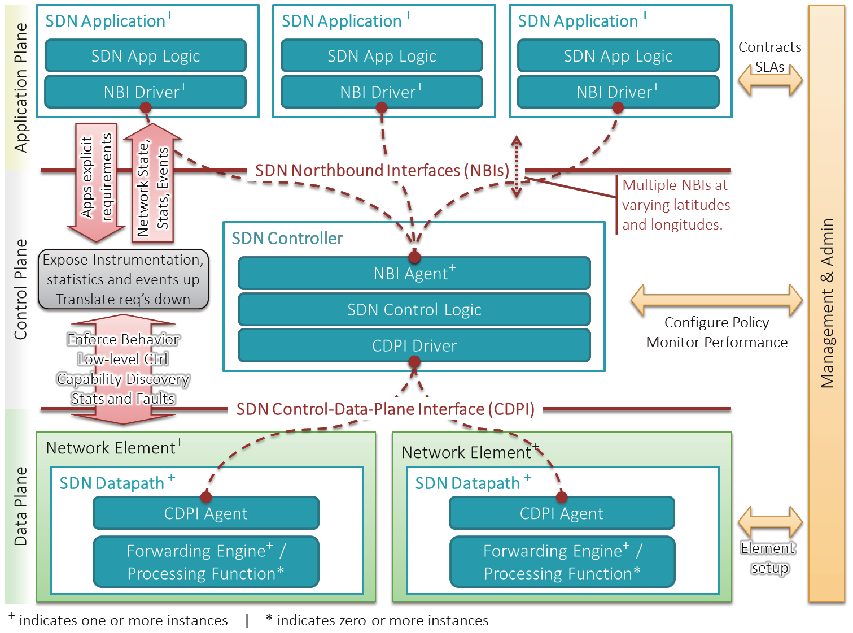
\includegraphics{arch/sdn-arch.pdf}
  \caption{软件定义网络SDN架构}
  \label{fig:pard-arch-outline}
\end{figure}


\section{本章小结}

本章首先介绍了本文的研究背景与问题,
即新计算模式下数据中心面临应用服务质量与资源利用率相冲突的问题,
并从软件和硬件两个角度总结针对该问题的相关研究。
从现有技术来看,单节点内服务质量保障技术的不足,导致节点内应用相互干扰严重,
已经成为目前数据中心整体服务质量保障的短板,是成为长尾延迟现象的主要因素之一。
单纯从软件或硬件层次无法根本解决该问题,而是需要跨层次协同设计。
而软硬件协同设计的关键在于``应用如何表达服务质量(QoS)目标并且让底层的硬件、操作
系统以及虚拟层共同工作来保障它们''\cite{21st_architecture}。
本文后续章节将围绕这一问题讨论如何设计一种新型的体系结构,
通过软硬件协同的方式解决数据中心当前面临的这一难题。

